\subsection{Logbog (Magnus)}
Logbogen var et dokument i Google Docs, der blev opdateret under de fysisker møder.
Logbogens primære formål var at:

\begin{enumerate}
\item Gøre det tydeligt, hvordan dagens opgaver var opdelt
\item Give et mere detaljeret overblik end commit messages i Git
\item Samle spørgsmål, der senere skulle drøftes som gruppe
\end{enumerate}

Farvekoder blev gerne brugt til at markere, at en opgave er blevet løst. Hensigten med at samle spørgsmål “til senere” var at opretholde workflowet, og i stedet tage overvejelser som fx datohåndtering op i logbogskrivningsfasen.

\begin{figure}[H]
    \centering
    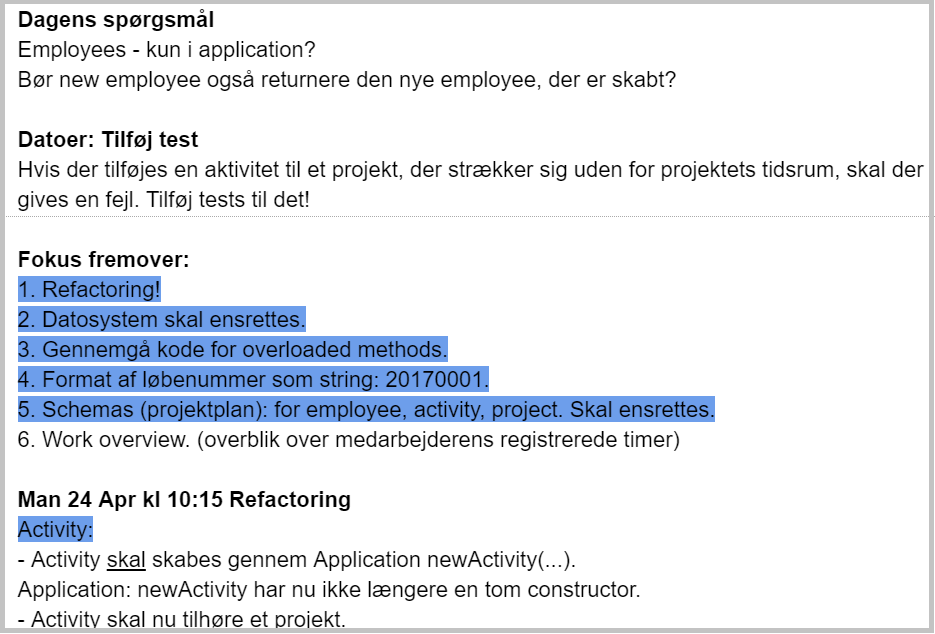
\includegraphics[width = 0.8\textwidth]{Figurer/logbog.PNG}
    \caption{Uddrag fra logbogens afsnit “Man 17 Apr implementering 1”, der dokumenterede første implementeringfase.}
\end{figure}
